\documentclass[a4paper,12pt,openright,titlepage,oneside]{book}

%\usepackage[english,brazil]{babel} 
%Define regra de gramática para separar síbalas {babel}
%e altera os títulos (como chapters, sections, references) para português
\usepackage[brazil]{babel}
% Define uso de caracteres acentuados no PDF gerado
% e permite copiar corretamente o texto do PDF.
\usepackage[T1]{fontenc}
\usepackage[utf8]{inputenc}

% Adição do pacote do template da UnB
\usepackage{template-FT-UnB/ft2unb}
\usepackage{booktabs}

\DeclareGraphicsExtensions{.jpg,.pdf,.mps,.png,.gif, .eps}
\graphicspath{imagens} %define diretório de imagens

%Arquivo com lista com hifenização correta de algumas palavras.
%Defina novas palavras no arquivo a medida que verificar que a hifenização automática
%etá errada para tais palavras.
%----------------DEFINE FORMA CORRETA DE HIFENIZAÇÃO PARA ALGUMAS PALAVRAS ----------------
\hyphenation{cons-tru-a}
\hyphenation{e-xem-plo}
\hyphenation{e-xem-plar}
\hyphenation{e-le-men-to}
\hyphenation{e-le-men-tar}
\hyphenation{ma-nu-al}
\hyphenation{res-pos-ta}
\hyphenation{ca-rac-te-ris-ti-ca}
\hyphenation{ca-rac-te-ris-ti-cas}
\hyphenation{ca-rac-te-ris-ti-co}
\hyphenation{ca-rac-te-ris-ti-cos}
\hyphenation{cor-res-pon-den-ci-as}
\hyphenation{cons-tru-am}
\hyphenation{re-a-li-za-da}
\hyphenation{re-a-li-za-do}
\hyphenation{re-a-li-za-das}
\hyphenation{re-a-li-za-dos}
\hyphenation{i-ne-xis-ten-cia}
\hyphenation{i-ne-xis-te}
\hyphenation{e-xis-te}
\hyphenation{di-fe-ren-te}
\hyphenation{di-fe-ren-tes}
\hyphenation{dei-xan-do}
\hyphenation{ins-ta-la-do} 
\hyphenation{ins-ta-la-dos} 
\hyphenation{ins-ta-la-da}
\hyphenation{ins-ta-la-das}
\hyphenation{re-gis-tra-do}
\hyphenation{re-gis-tra-dos}
\hyphenation{re-gis-tra-da}
\hyphenation{re-gis-tra-das}
\hyphenation{des-cre-ve}
\hyphenation{res-pei-to}
\hyphenation{re-a-li-za}
\hyphenation{re-a-li-zar}
\hyphenation{a-tu-a-li-zar}
\hyphenation{a-tu-a-li-zan-do}
\hyphenation{a-tu-a-li-za-do}
\hyphenation{a-tu-a-li-za-da}
\hyphenation{fun-ci-o-na-li-da-de}
\hyphenation{pos-si-bi-li-da-de}
\hyphenation{dis-po-si-ti-vo}
\hyphenation{dis-po-si-ti-vos}
\hyphenation{e-xis-te}
\hyphenation{e-xis-tir}
\hyphenation{des-co-ber-ta}
\hyphenation{des-co-ber-to}
\hyphenation{de-sig-nar}
\hyphenation{de-sig-na-do}
\hyphenation{o-pe-ra-ci-o-nais} 
\hyphenation{o-pe-ra-ci-o-nal}
\hyphenation{con-si-de-ra-do}
\hyphenation{con-si-de-ra-dos}
\hyphenation{ou-tro}
\hyphenation{ou-tra}
\hyphenation{ou-tros}
\hyphenation{ou-tras}
\hyphenation{e-xis-ten-te}
\hyphenation{e-xis-ten-tes}
\hyphenation{LuaOnTV}
\hyphenation{De-fi-ni-tion}
%------------------------------------------------------------------------------------------ 

% ALTERE OS VALORES DENTRO DAS CHAVES DOS COMANDOS NESTA SEÇÃO PARA INCLUIR OS SEUS DADOS E DADOS DA SUA
% DISSERTAÇÃO DE MESTRADO OU TESE DE DOUTORADO
% -----------------------------------------------------------------------------------------------------

%\onehalfspacing
\title{Projeto de EPS para um Nanossatélite CubeSat}
\author{Hugo Nascimento Fonseca}
\date{2020-06-XX} %data da defesa

\grau{Engenheiro} %Mestre ou Doutor
\area{Engenharia de Computação} %Nome do curso
\siglaarea{ENE} %Sigla do departamento
\tipodemonografia{Trabalho} %Dissertação ou Tese
\programa{Graduação} %Mestrado ou Doutorado
\autorendereco{QNM 03 Conjunto I Casa 26} %Endereço do autor da dissertação/tese
\totalpgs{147} %total de páginas atualmente na sua dissertação
\dia{XX} %dia da defesa
\mes{Junho} %mês da defesa
\ano{2020} %ano da defesa
\numpublicacao{xxx/AAAA} %número da publicação (após a defesa, tal número deve ser obtido na secretaria)

%PPGENE.DM  = Programa de Pós Graduação em ENgenharia Elétrica.Dissertação de Mestrado
%PPGENE.TD  = Programa de Pós Graduação em ENgenharia Elétrica.Tese de Doutorado
\siglapublicacao{PPGENE.DM}

\titulolinhai{PROJETO DE EPS para um}
\titulolinhaii{Nanossatélite CubeSat}
\titulolinhaiii{}
\titulolinhaiv{}

\autori{HUGO NASCIMENTO FONSECA}
%Caso seu nome não caiba em uma única linha, divida ele nos comandos abaixo
%\autorii{} 
%\autoriii{}

\membrodabancai{Prof. Dr. Daniel Chaves Café, ENE/UnB}
\membrodabancaifuncao{Orientador}
\membrodabancaii{Prof. Fulano de Tal 2, ENE/UnB}
\membrodabancaiifuncao{Examinador interno}
\membrodabancaiii{Prof. Fulano de Tal 3, ENE/UnB}
\membrodabancaiiifuncao{Examinador interno}
\membrodabancaiv{Prof. Fulano de Tal 4, EESC/USP}
\membrodabancaivfuncao{Examinador externo}
\membrodabancav{}
\membrodabancavfuncao{}
% -----------------------------------------------------------------------------------------------------

%line-numbers, inputencoding=utf8/latin1
%Define o estilo para listagens de código fonte
\lstset{
  numbers=left, %numeração de linhas à esquerda
  stepnumber=1,
  firstnumber=1,
  numberstyle=\tiny,
  extendedchars=true,
  frame=none,
  basicstyle=\footnotesize,
  stringstyle=\ttfamily,
  showstringspaces=false,
  %language=Java, %deve ser definida na inclusão de cada trecho de código, pois podem existir linguagens diferentes em exemplos diferentes
  breaklines=true,
  breakautoindent=true,
  %estilos de comentário de uma e várias linhas
  morecomment=[l]{--}, morecomment=[s]{/*}{*/}, morecomment=[s]{<!--}{-->}, morecomment=[s]{--[[}{--]]}
}

% Adição de metadados no PDF (propriedades do documento PDF)
\makeatletter
	 \hypersetup{
		 pdftoolbar=true,        % show Acrobat’s toolbar?
		 pdfmenubar=true,        % show Acrobat’s menu?
		 pdffitwindow=false,     % window fit to page when opened
		 pdfstartview={FitH},    % fits the width of the page to the window	 
		 pdftitle={\@title},
		 pdfauthor={\@author},
		 pdfsubject={\tipodemonografianome \ de\ \programastr \ em\ \areastr},   % subject of the document
		 pdfcreationdate={\pdfdate}
	 }
\makeatother


\makeindex
\makenomenclature %Necessário para gerar lista de siglas


\begin{document}

	\pdfbookmark[0]{Agradecimentos}{agradecimentos}
	%* indica para nao adicionar numeracao ao titulo
\chapter*{Agradecimentos}

Agradeço, primeiramente, à minha família que foi a base para que tudo isso fosse possível. Agradeço o meu orientador Prof. Dr. Daniel Chaves Café que sempre me incentivou e acompanhou, com muito tato e compreensão, as dificuldades que superamos juntos nesse ano de pandemia. E por fim, agradeço os meus amigos e colegas de curso, especialmente os da Struct - Empresa Júnior de Engenharia de Computação, lugar onde aprendi muito e me trouxe diversas oportunidades de crescimento. 
	\chapter*{Resumo}
O presente trabalho apresenta um estudo de viabilidade e ao final propõe uma versão para o desenvolvimento de um dispositivo EPS, sigla para \textit{Electrical Power System}, para um \textit{Cubesat} 1U. O objetivo consiste em propor uma placa eletrônica que realize a aquisição, armazenamento e distribuição de energia, além de atender os demais requisitos da missão em diversas frentes, tais como a padronização, as conexões com os sistemas embarcados necessários, os requisitos de operação, o consumo, entre outros. Será apresentado em detalhes um \textit{background} com missões anteriores, de outras universidades do mundo inteiro, alguns conceitos teóricos necessários e, por fim, o hardware proposto para o projeto. Esse trabalho está inserido no contexto do projeto Alfa Crux, desenvolvido pelo laboratório LODESTAR, Laboratório de Simulação e Controle de Sistemas Aeroespaciais, da Universidade de Brasília (UnB), que tem como um de seus objetivos desenvolver uma constelação de nanossatélites, sendo o primeiro lançamento previsto para até o final de 2021, início de 2022. 

\textbf{\textit{Keywords}: Cubesat, nanossatélite, EPS, MPPT, microcontrolador, conversão, DC-DC}

	
	\pdfbookmark[0]{Sumário}{sumario}
	\sumario
	
	\pdfbookmark[0]{Lista de Figuras}{listafiguras}
	\listadefiguras
	
	\pdfbookmark[0]{Lista de Tabelas}{listatabelas}
	\listadetabelas
	
	\pdfbookmark[0]{Lista de Códigos Fonte}{listacodigosfonte}
	\listadecodigosfonte
	
	\renewcommand{\nomname}{LISTA DE TERMOS E SIGLAS} %Define um caption à lista de siglas
	%Inclui a lista de siglas 
	\pdfbookmark[0]{Lista de Termos e Siglas}{nomenclatura}
	\printnomenclature[2.5cm] 
	
	\mainmatter %Inicia a numeracao normal cardinal
	\setcounter{page}{1} \pagenumbering{arabic} \pagestyle{plain}
	
	% Lista de termos e siglas
\nomenclature{ADC}{\textit{Analog to Digital Converter} - Conversor Analógico Digital}
\nomenclature{ADCS}{\textit{Attitude Determination and Control System} - Sistema de Determinação e Controle de Atitude}
\nomenclature{BJT}{\textit{Bipolar Junction Transistor} - Transistor Bipolar de Junção}
\nomenclature{COTS}{\textit{Commercial Off-The-Shelf} - Comercial pronto para uso}
\nomenclature{EPS}{Electrical Power System - Sistema Elétrico de Potência}
\nomenclature{MCU}{Microcontrolador}
\nomenclature{MOSFET}{\textit{Metal-Oxide-Semiconductor Field Effect Transistor} - Transistor de Efeito de Campo Metal - Óxido - Semicondutor}
\nomenclature{MPPT}{\textit{Maximum Power Point Tracking} -  Rastreamento do Ponto de Máxima Potência}
\nomenclature{OBC}{\textit{On-board computer} - Computador de bordo}
\nomenclature{PCB}{\textit{Printed Circuit Board} - Placa de circuito impresso}
\nomenclature{PWM}{\textit{Pulse Width Modulation} - Modulação por largura de pulso}
\nomenclature{RBF}{\textit{Remove Before Flight} - Remover Antes do Voo}
\nomenclature{UnB}{Universidade de Brasília}
	\chapter{Introdução} \label{introducao}
\section{Contextualização}
Satélite é um termo utilizado para qualquer objeto que gira em torno de um corpo celeste em função da ação da força gravitacional. Ao longo dos anos, com o avanço da tecnologia, a humanidade desenvolveu e construiu centenas de milhares de satélites artificiais para cumprir diversos tipos de missões, por exemplo, aquisição de dados, monitoramento, posicionamento, telecomunicações, demonstrações, estudos meteorológicos, entre outros. Diariamente, milhões de pessoas consomem serviços que estão, direta ou indiretamente, relacionados com o funcionamento de algum satélite, não há dúvidas que os satélites artificiais permitiram que o mundo se tornasse uma grande aldeia.

Satélite artificial é qualquer dispositivo projetado para funcionar no espaço orbital da Terra, sendo que a principal variável a ser definida no desenvolvimento de um satélite é a sua missão, pois ela que guia boa parte das escolhas do projeto - órbita utilizada, formato, funcionalidades, tempo de vida, entre outras. Porém, para que esses dispositivos consigam prover alguma utilidade, todos têm uma infraestrutura em comum, o que inclui comunicação de dados, suprimento de energia, cálculo de posição, isso além das suas funções customizadas.\cite{nasa_comms_article} 

Este trabalho de conclusão de curso é um memorial de projeto de um EPS para o nanossatélite do projeto Alfacrux. O projeto é uma iniciativa de pesquisadores e alunos da Universidade de Brasília (UnB) que irá colocar em órbita baixa (aproximadamente 500 km de altitude) um nanossatélite até o final de 20XX.

O projeto Alfacrux tem como um de seus objetivos desenvolver um nanossatélite de comunicação em ondas curtas, ou seja, será possível trafegar sinais de voz e dados, porém em baixo volume, uma vez que o foco será prover comunicação em longo alcance para atingir áreas remotas. O nanossatélite será operado pela UnB atráves de bases em solo durante sua vida útil estimada de aproximadamente 2 anos, esse projeto é uma plataforma de interesse estratégico de parceiros como o Exercíto Brasileiro, uma vez que ele poderá ser utilizado, por exemplo, para fornecer comunicações em regiões remotas, a exemplo da Amazônia, onde não se tem infraestrutura ou interesse econômico em ofertar o serviço. 

Juntamente com o desenvolvimento do projeto, nos objetivos acadêmico-científicos, deseja-se criar uma base sólida de documentação, do qual esse trabalho faz parte, para consolidar, registrar e propagar a enorme carga de conhecimento gerada pelos participantes do projeto.

\section{Objetivos}
\subsection{Gerais}\label{gerais}
% Descrever a necessidade do projeto da placa, seguindo o formato CubeSat, etc...

O Sistema Elétrico de Potência (EPS) é um subsistema vital para o funcionamento do \textit{CubeSat}, uma vez que ele é responsável por toda a gestão da energia do satélite. Normalmente, ele é dividido em duas partes principais, sendo uma responsável pelo carregamento da bateria atráves de panéis solares e uma segunda parte de que faz a regulação e distribuição das linhas de tensão necessárias para os demais módulos. 

O objetivo geral desse trabalho é desenvolver uma placa eletrônica que atue como EPS do nanossatélite Alfacrux, respeitando as demandas enumeradas abaixo:

\begin{enumerate}
    \item Possuir proteção contra \textit{undervoltage} e \textit{overvoltage} da bateria
    \item Possuir proteção contra \textit{overcurrent} na linhas reguladas
    \item Possuir sistema que maximiza a potência da placa solar, mais detalhes na seção \ref{mppt_revision}
    \item Possuir baterias para manter o satélite alimentado durante os períodos de eclipse
    \item Possuir controle de quais linhas estão ligadas
    \item Possuir interface de comunicação com OBC - Computador de bordo
    \item Permitir desenvolvimentos futuros
    \item Estar em concordância com o padrão \textit{CubeSat}, mais detalhes na seção \ref{cubesat_revision}
\end{enumerate}{}


\subsection{Específicos}\label{especificos}
% Reunião prof. Café: 
% Colocar com deliverables os levantamentos (consumo, processamento, interfaces)
% Entregavel: lista de especificações de projeto
Objetivos específicos (tarefas/deliverables para o TCC 2)
\begin{enumerate}
    \item Levantamento dos requisitos de consumo
    \item Levantamento das tarefas do nanossatélite
    \item Dimensionar a demanda de energia conhecendo o consumo esperado e as tarefas desempenhadas pelos módulos
    \item Levantamento das interfaces necessárias (entre a própria placa e também com outros sistemas do nanossatélite)
    \item Levantamento das condições de operação
    \item Lista de especificações e componentes escolhidos para o projeto
    \item Simulações dos circuitos do EPS
    \item Projeto da PCB
\end{enumerate}

	\chapter{Revisão Teórica} \label{revisão}
% [Futuramente, pode ser necessário expandir essa seção]

Esta seção visa oferecer os conceitos necessários para o completo entendimento desse trabalho. Inicialmente, serão apresentados os conceitos relacionados a classificação de satélites, o padrão CubeSat, alguns conceitos de eletrônica e, por fim, um histórico das missões anteriores com enfoque nos sistemas de potência utilizados.

\section{Nanosatélites}\label{nanosats_revision}
Normalmente, a classificação mais utilizada para satélites é com relação a sua massa. Na figura abaixo, podemos ver as categorias utilizadas nessa classificação e alguns exemplos de artefatos já lançados. Observe que os nanossatélites se encontram na faixa de 1 até 10 kg.

\noindent
\begin{minipage}{\linewidth}
\makebox[\linewidth]{
    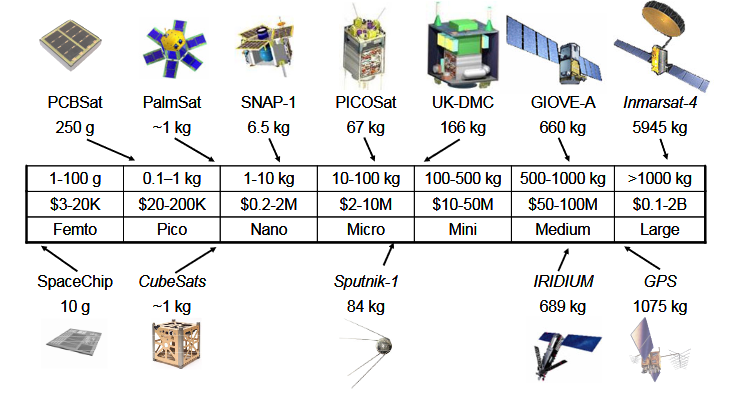
\includegraphics[keepaspectratio=true, scale=0.5]{imagens/Satellite-mass-classification.png}}
\label{mass_classification_fig}
\captionof{figure}{Classificação de satélites, com alguns exemplos}
\end{minipage}

 Os principais responsáveis por essa redução de massa são a miniaturização dos circuitos integrados e as padronizações das estruturas de lançamento, como no padrão \textit{Cubesat}. Os nanossatélites são amplamente utilizados nas atividades de ensino, pois permitem um ciclo completo de uma missão espacial mantendo um custo baixo, principalmente devido ao uso de peças comerciais.\cite{barnhart_ref}

\section{\textit{Cubesat}}\label{cubesat_revision}

O padrão \textit{Cubesat} foi um dos grandes responsáveis pela popularização da categoria de nanossatélites, como podemos ver no gráfico abaixo, que mostra o número de lançamentos desse tipo por ano.\cite{cubesats_cgee}.

\noindent
\begin{minipage}{\linewidth}
\makebox[\linewidth]{
    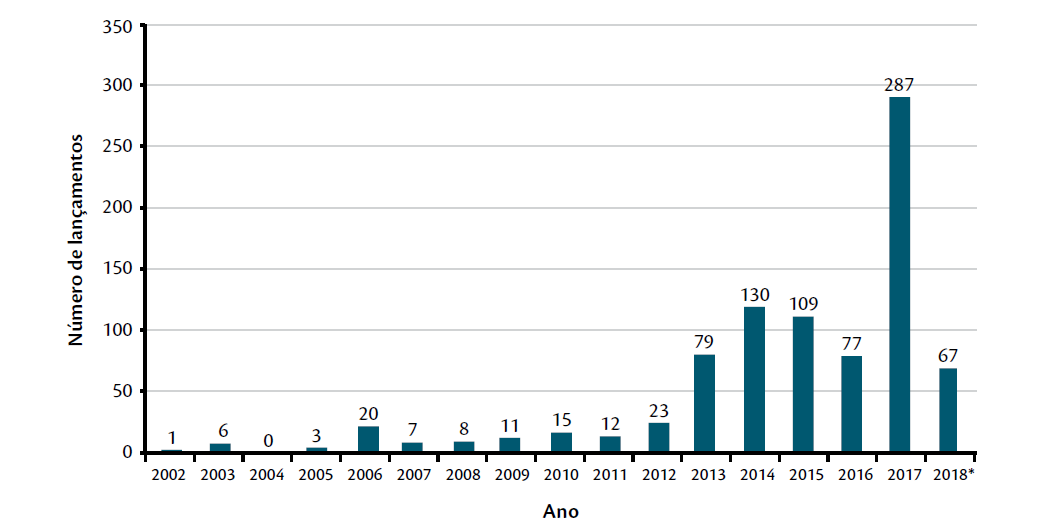
\includegraphics[keepaspectratio=true, scale=0.5]{imagens/cubesat-launches-count.png}}
\captionof{figure}{Distribuição do número de \textit{Cubesats} pelo ano de lançamento}
\label{cubesat_launches_fig}
\end{minipage}

O modelo \textit{Cubesat} foi proposto em 1999 por Jordi Puig-Suari, da \textit{California Polytechnic State University}, e Bob Twiggs, da \textit{Stanford University}. O objetivo era um modelo de satélite de pequeno porte que segue um padrão mais simples, o intuito deles era fornecer aos alunos de ambas universidades a oportunidade de  participar de um projeto espacial completo, incluindo todas as fases, desde a construção, testes e operação do artefato, que manteria características similares aos satélites maiores. 

O termo é um acrônimo entre as palavras \textit{cube} (em inglês, cubo) acrescida das três primeiras letras da palavra satélite.

Normalmente, as missões com \textit{Cubesats} tem um risco técnico mais elevado, em parte devido ao uso de componentes não \textit{"space qualified"}, porém oferecem em troca uma implementação mais rápida, aplicações mais inovadoras, custos menores ou um conjunto desses elementos.

As principais características dos \textit{Cubesats} são as seguintes:
\begin{itemize}
    \item compostos por unidades cúbicas padronizadas (1U) de tamanho 10x10x10 cm, conforme mostrado na figura \ref{cubesat_configs_fig};
    \item uso de sistemas padronizados de ejeção em órbita, denominados, P-POD (do inglês, \textit{Poly Picosatellite Orbital Deployer}) ou SSPL (do inglês, \textit{Space Shuttle Picosatellite Launcher}). Esses sistemas são capazes de liberar diversos satélites pela mesma interface;
    \item componentes COTS nos sistemas de bordo.
\end{itemize}

\noindent
\begin{minipage}{\linewidth}
\makebox[\linewidth]{
    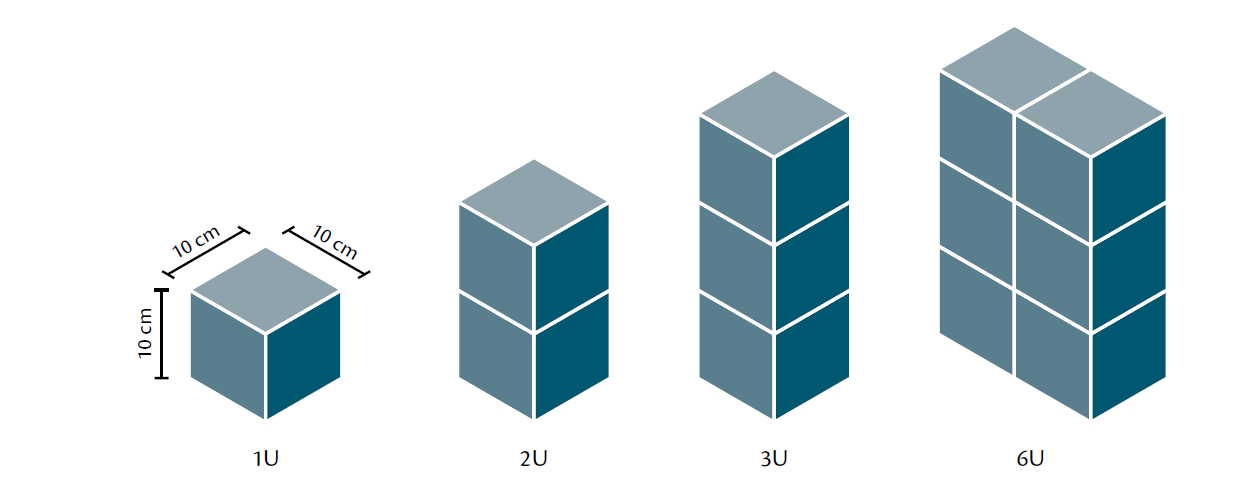
\includegraphics[keepaspectratio=true, scale=0.5]{imagens/cubesats-configs.png}}
\captionof{figure}{Algumas configurações de \textit{Cubesats}}
\label{cubesat_configs_fig}
\end{minipage}

O padrão é descrito em um documento de domínio público\cite{cubesat_specs_rev13}, onde especifica-se que uma unidade \textit{Cubesat} ou 1U, tem um volume de 1 litro e carga útil de até 1,3 kg, podendo combinar várias unidades dessas para compor satélites maiores (2U, 3U, 6U ou 12U, por exemplo).

Quanto aos requisitos elétricos, o padrão apresenta dois requisitos extremamente importantes que são o \textit{Deployment Switch} e o pino \textit{Remove Before Flight} (RBF).
\begin{enumerate}
    \item O \textit{Deployment Switch} é uma chave que deve desconectar eletricamente todos os subsistemas, sem exceções, do sistema de potência.
    \item Essa chave deve atuar durante todo o tempo que o CubeSat estiver acoplado no P-POD, e esse sinal é recebido dos trilhos do P-POD, conforme figura X.
    \item Por sua vez, o RBF, é um pino que deve cortar toda a alimentação do satélite uma vez que estiver inserido. Ele será removido após o encaixe na base de lançamento P-POD e não deve avançar mais do que 6.5 mm além dos trilhos.
\end{enumerate}

\noindent
\begin{minipage}{\linewidth}
\makebox[\linewidth]{
    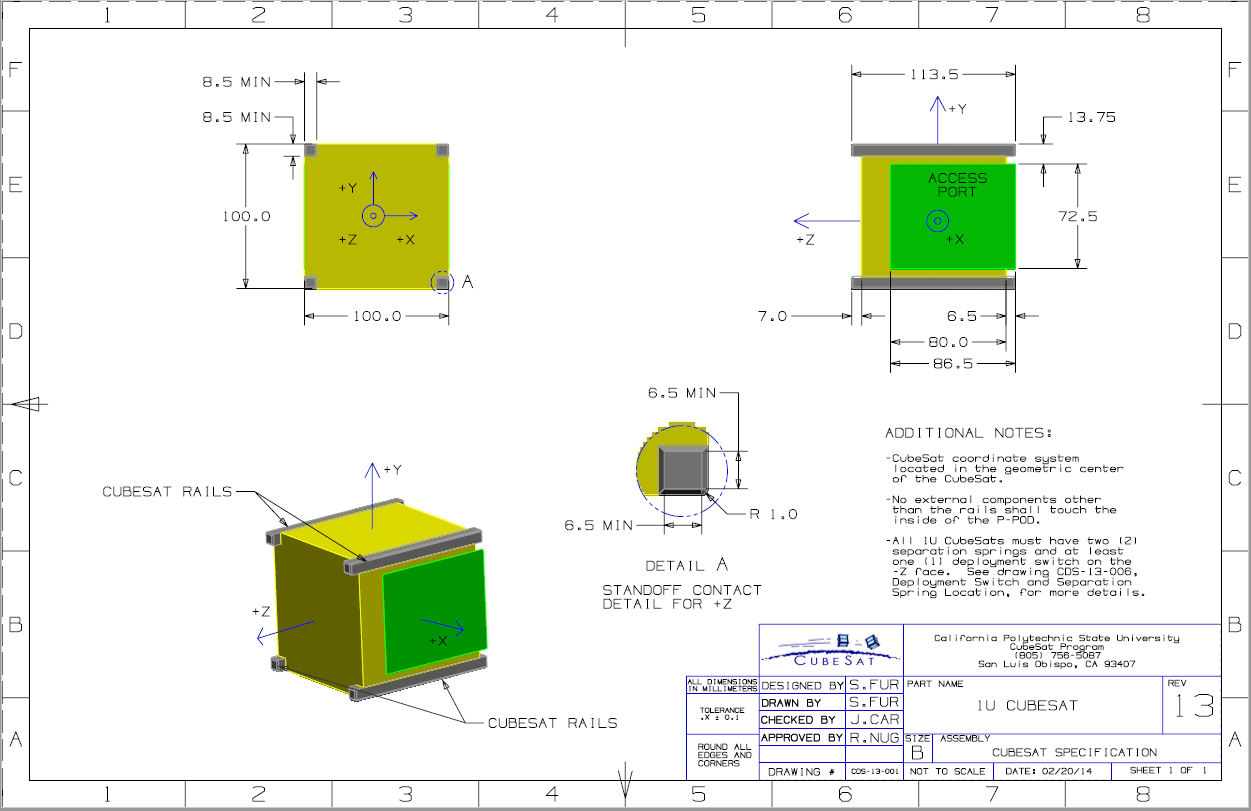
\includegraphics[keepaspectratio=true, scale=0.5]{imagens/Cubesat-diagram.png}}
\captionof{figure}{Especificações de dimensionamento para um \textit{Cubesat} 1U}
\label{cubesat1U_dimensions_fig}
\end{minipage}

Por esses e outros aspectos, os \textit{Cubesats} trouxeram um aspecto inovador capaz de mudar o paradigma do setor espacial, adequando-o à nova tendência de emprego de pequenos satélites para atender a diferentes tipos de demandas.

\section{Printed Circuit Board (PCB)}\label{pcb_revision}
\textit{Printed Circuit Board}, em português: placa de circuito impresso, é uma técnica amplamente utilizada na eletrônica que consiste em construir uma placa de um material isolante que apresenta em sua superfícies trilhas condutoras que representam o circuito em que serão soldados os dispositivos eletrônicos.

Para a maioria dos circuitos, ter apenas uma superficie condutora é insuficiente dado que algum momento durante o design será impossível evitar o cruzamento entre trilhas, portanto, a maioria das PCBs são multicamadas, ou seja, possuem múltiplas camadas de trilhas condutoras isoladas.

Essa forma de construir circuitos representou grande avanço na eletrônica, pois esse arranjo permite maior resistência a interferências, melhor fixação dos componentes e otimização no uso do espaço, possibilitando equipamentos menores.

O processo moderno de design de uma PCB é facilitado pelo uso de software de \textit{layout} dedicado que ao final do processo nos fornece os arquivos .gerber que serão usados para a fabricação, nesses arquivos não são colocadas informação sobre os componentes, há apenas as informações que o fabricante da PCB necessita, a exemplo das \textit{layers}, furações, entre outros.

\section{Conversores DC-DC}\label{converters_revision}
\subsection{Topologia Buck}
\subsection{Topologia Boost}
\subsection{Topologia Buck-Boost}
\subsection{Topologia SEPIC}

\section{MPPT - Maximum Peak Point Tracking}\label{mppt_revision}
\subsection{Algoritmo: Pertuba e Observa}
\subsection{Algoritmo: Condutância Incremental}

\subsection{Ambiente espacial}
Um problema a ser considerado no desenvolvimento, especialmente das placas eletrônicas, é o efeito do ambiente espacial nos subsistemas. Os problemas causados podem variar desde mal funcionamento até danos físicos, normalmente essas considerações são feitas para missões de longa duração realizadas em \textit{LEO} (do inglês \textit{Low Space Orbit}) e \textit{Deep Space} \cite{nasa_state_of_art}.

A quantidade de radiação que incide nos satélites depende da altitude e do tipo da órbita. A maioria dos \textit{Cubesats} são colocados em órbitas LEO (entre 100 e 1000 km de altitude), recebendo uma dose de radiação de  aproximadamente 0,1 krad/ano.

A resistência a radiação é um dos grandes desafios das missões \textit{Cubesat}, pois os componentes COTS não tem nenhuma preocupação com radiação durante o processo de design, logo, os clientes desses componentes devem blindar todas as partes eletrônicas, realizar todos os testes de exposição e assumir os possíveis riscos de falhas.

\section{Microcontrolador/Microprocessador}\label{mcu_revision}
A principal diferenciação entre microcontroladores e microprocessadores está na quantidade de componentes que estão embarcados em um e outro. O microcontrolador (MCU) é um computador completo inteiro em um único circuito integrado, ou seja, contém memórias, timers, portas de comunicação serial, entre outros periféricos. Já o microprocessor contém essencialmente as unidades de controle e cálculo, necessitando de periféricos externos para formar um sistema minímo de um computador.

Os MCUs atualmente encontram uma enorme gama de aplicações na eletrônica moderna, desde máquinas industriais, sistemas embarcados a brinquedos e eletrodomésticos. São exemplos de microcontroladores: Texas Instruments MSP430, PIC, Atmel AVR, ARM Cortex-M, entre outros.

Para a nossa missão, a escolha do MCU é um ponto-chave, uma vez que ele é o componente mais importante do OBC, pois é o responsável por executar o \textit{software} destinado ao gerenciamento do satélite. Abaixo seguem alguns critérios importantes na escolha do MCU mais adequado:

\begin{enumerate}
    \item Baixo consumo: a disponibilidade de energia em órbia dependerá da área de cobertura e eficiência dos painéis solares e essa potência também será dividida com os outros subsistemas, logo, o nosso MCU tem que consumir pouco quando em funcionamento;
    \item Conversores AD: O OBC necessitará ler dados de muitos sensores, exemplo: temperatura e luminosidade;
    \item Portas I/O: As portas GPIO (do inglês \textit{General-Purpose Input/Output}) são essenciais para comunicação com os outros subsistemas;
    \item Interfaces Seriais: Ter pinos dedicados aos protocolos de comunicação serial (UART, I2C, SPI) ajudam no desenvolvimento do OBC;
    \item PWM: Para o controle de motores, consequentemente há necessidade de pinos que produzam PWM;
    \item Frequência de Operação: Deseja-se usar um microcontrolador com uma frequência de \textit{clock} elevada para ter uma melhor performance;
    \item Faixa de temperatura: O microcontrolador deve resistir a qualquer temperatura encontrada na órbita LEO.
\end{enumerate}

Mais adiante, no capítulo de desenvolvimento (\ref{desenvolvimento}) abordaremos a nossa escolha de microcontrolador e como esses e outros critérios foram avaliados.


\section{Histórico de missões anteriores}\label{missions_history}

Um levantamento de trabalho com escopo semelhante a este foi realizado e a Tabela \ref{history_table} mostra alguns exemplos de \textit{CubeSats}, indicando a missão, o tamanho, ano de deploy e quais as soluções utilizadas.

\begin{table}
\centering
\caption{Missões anteriores com \textit{Cubesats}}
\label{history_table}
\begin{tabular}{|l|l|l|l|} 
\hline
\multicolumn{1}{|c|}{Nome} & \multicolumn{1}{c|}{Tipo} & \multicolumn{1}{c|}{Ano} & \multicolumn{1}{c|}{Implementação do EPS}  \\ 
\hline
Cute 1.7+                  & Demonstração              & 2008                     &  Implementação do MPPT, centralizado  \\ 
\hline
SNAP-1                     & Demonstração              & 2000                     &  Implementação do MPPT, parcialmente distribuído  \\
\hline
ESTCube-1                  & Científico                & 2013                     &  Controladores MPPT, centralizado     \\ 
\hline
SwissCube                  & Observação                & 2009                     &  Implementação do MPPT, centralizado  \\
\hline
\end{tabular}
\end{table}

O CUTE \cite{cute1_ref} (Cubical  Tóquio  Tech  Engineering  Satellite-I) é um projeto cooperativo do LSS (Laboratory for Space Systems) e o SRTL (Space Robotics and Teleoperations Laboratory), ambos de Tóquio. O computador de bordo foi implementado com um processador Hitachi NPD-20JWL e executava o sistema operacional Windows CE.NET. O  projeto  educacional  de  baixo  custo  usava componentes COTS para uma missão de demonstração tecnológica, o projeto teve diversões lançamentos (Cute-I, Cute 1.7+ APD, Cute 1.7+ APD II). 

O SNAP-1 \cite{snap1_ref} foi o primeiro nanossatélite desenvolvido no Reino Unido pela Surrey Space Centre (SSC) e Surrey Satellite Tecnology Ltd (SSTL) e serviu como veículo de teste para demonstração da nova tecnologia que estava surgindo, ele foi um dos pioneiros dessa nova filósofia de design e mostrou que era possível construir um nanossatélite rapidamente e com custo baixo, utilizando peças COTS.

SamSat-218D \cite{samsat218_ref} foi um nanossatélite desenvolvido na \textit{Samara State Aerospace University}, lançado em 2015, e foi criado com o objetivo de ser uma plataforma de testes para tecnologias de navegação e controle. Além disso, o projeto foi utilizado para testar um OBC experimental, que empregava os processadores ATXmega 128U4 e LPC4357 DualCore, testar o controle de voo em condições anormais e novos painéis solares.

ESTCube-1 \cite{estcube1_ref} foi um \textit{cubesat} 1U lançado pelo foguete Vega VV02. Desenvolvido por uma força tarefa de 4 universidades, tinha o objetivo científico de realizar um prova de conceito de medição e demonstração da tecnologia da tecnologia de velas solares elétricas. Para o OBC um STMicroelectronics STM32F103 (ARM 32bits) foi escolhido para fazer os cálculos.

Cat-2 \cite{cat2_ref} foi um projeto de \textit{cubesat} 6U desenvolvido na \textit{Universitat Politècnica de Catalunya} e iniciado em 2009 para lançar um nanossatélite plataforma para um instrumento GNSS-R (do inglês, \textit{Global Navigation Satellite Systems Reflectometry}) que realizaria altimetria oceânica. A computação de bordo ficou a cargo de um ARM7TDMI.  

O SwissCube-1, \cite{swisscube_ref} foi um \textit{cubesat} suíço científico de tamanho 1U, operado pela Ecole Polytechnique Fédérale de Lausanne (EPFL) para realizar pesquisas sobre o \textit{nightglow} (fenômeno de brilho   noturno na atmosfera terrestre) e também para desenvolver tecnologia para futuras naves espaciais. A  computação  de  bordo utilizava um processador ARM7TDMI e o sistema operacional de tempo real FreeRTOS.

% Segundo \cite{soares2007ginga}:

% \begin{quote}
% 	Lorem ipsum dolor sit amet, consectetuer adipiscing elit. Ut purus elit, vesti- bulum ut, placerat ac, adipiscing vitae, felis. Curabitur dictum gravida mauris. Nam arcu libero, nonummy eget, consectetuer id, vulputate a, magna. 
% \end{quote}

% \lstset{caption=Exemplo de aplicação servidora, label=list:server}
% \begin{lstlisting}[language=C]
% int main()
% { 
%     FILE *fp;     int len;     
%     static const int SIZE = 1024;
%     struct sockaddr_in me, target;
%     int sock=socket(AF_INET,SOCK_DGRAM,0);
%     char arquivo[SIZE];
%     me.sin_family=AF_INET;
%     me.sin_addr.s_addr=htonl(INADDR_ANY); // endereco IP local 
%     me.sin_port=htons(0); // porta local (0=auto assign)
%     bind(sock,(struct sockaddr *)&me,sizeof(me));
%     target.sin_family=AF_INET;
%     target.sin_addr.s_addr=inet_addr("192.168.68.217"); // host local 
%     target.sin_port=htons(8450); // porta de destino 

%     if ((fp = fopen("video1.mp4","rb")) == NULL){
%         printf("Arquivo nao pode ser aberto.\n"); return -1;
%     }

%     while(!feof(fp)) {
%         len = fread(arquivo, 1, sizeof(arquivo), fp);
%         sendto(sock,arquivo,sizeof(arquivo),0,(struct sockaddr *)&target,sizeof(target));
%     }
%     sendto(sock,"FIM",sizeof("FIM"),0,(struct sockaddr *)&target,sizeof(target));
%     close(sock);
%     return 0;
% }
% \end{lstlisting}

	\chapter{Desenvolvimento} \label{desenvolvimento}

Antes de iniciar o desenvolvimento, foi realizada uma extensa pesquisa sobre missões com \textit{CubeSats} para buscar referências e teve por objetivo entender os requisitos e especificações de outras missões bem sucedidas e usar essas informações como um guia para o EPS que será desenvolvido no LODESTAR. 

A tabela \ref{history_table} mostra as missões, ano de deploy e um resumo das soluções utilizadas.

\begin{table}
\centering
\caption{Missões anteriores com \textit{Cubesats}}
\label{history_table}
\begin{tabular}{|l|l|l|l|} 
\hline
\multicolumn{1}{|c|}{Nome} & \multicolumn{1}{c|}{Tipo} & \multicolumn{1}{c|}{Ano} & \multicolumn{1}{c|}{Implementação do EPS}  \\ 
\hline
Cute 1.7+                  & Demonstração              & 2008                     &  Implementação do MPPT, centralizado  \\ 
\hline
SNAP-1                     & Demonstração              & 2000                     &  Implementação do MPPT, parcialmente distribuído  \\
\hline
ESTCube-1                  & Científico                & 2013                     &  Controladores MPPT, centralizado     \\ 
\hline
SwissCube                  & Observação                & 2009                     &  Implementação do MPPT, centralizado  \\
\hline
\end{tabular}
\end{table}

O CUTE \cite{cute1_ref} (Cubical  Tóquio  Tech  Engineering  Satellite-I) é um projeto cooperativo do LSS (Laboratory for Space Systems) e o SRTL (Space Robotics and Teleoperations Laboratory), ambos de Tóquio. O EPS utilizava 4 baterias de Li-ion e as células solares proviam em média 4 W, possuia linhas estabilizadas de 3.3, 5, 6 e 7 V. O  projeto  educacional  de  baixo  custo  usava componentes COTS para uma missão de demonstração tecnológica, o projeto teve outros lançamentos posteriores. (Cute-I, Cute 1.7+ APD, Cute 1.7+ APD II). 

O SNAP-1 \cite{snap1_ref} foi o primeiro nanossatélite desenvolvido no Reino Unido pela Surrey Space Centre (SSC) e Surrey Satellite Tecnology Ltd (SSTL) e serviu como veículo de teste para demonstração da nova tecnologia que estava surgindo, ele foi um dos pioneiros dessa nova filósofia de design e mostrou que era possível construir um nanossatélite rapidamente e com custo baixo, utilizando peças COTS. O seu EPS tem uma arquitetura parcialmente distribuida, porque das suas duas linhas de tensão (5 e 12 V), a de 12 V não é regulada, dessa forma, cada módulo que utilize essa linha deve implementar a regulação. Além disso, utiliza uma única bateria de 10 Wh e o EPS tem um modo burst, onde é possível utilizar até 60 W por alguns minutos.

ESTCube-1 \cite{estcube1_ref} foi um \textit{cubesat} 1U lançado pelo foguete Vega VV02. Desenvolvido por uma força tarefa de 4 universidades, tinha o objetivo científico de realizar um prova de conceito de medição e demonstração da tecnologia da tecnologia de velas solares elétricas. O seu EPS utilizava um design próprio um controlador MPPT da STMicroelectronics (SPV1040) para cada 4 células solares com duas baterias 18650 da Panasonic totalizando 9 Wh e linhas controladas de 12, 5 e 3.3 V.

O SwissCube-1, \cite{swisscube_ref}\cite{lessons_swisscube_ref} foi um \textit{cubesat} suíço científico de tamanho 1U, operado pela Ecole Polytechnique Fédérale de Lausanne (EPFL) para realizar pesquisas sobre o \textit{nightglow} (fenômeno de brilho noturno na atmosfera terrestre) e também para desenvolver tecnologia para futuras naves espaciais. O seu EPS utilizava um design próprio com duas baterias de 1200 mAh, uma única linha de tensão, controlada por um circuito analógico, de 3.3 V,  e possui um sistema de beacon integrado que funciona sem o auxilio de microcontroladores externos, como os do OBC, por exemplo.

\section{Análise de consumo energético da missão}

Um dos pontos centrais para um projeto de EPS é dimensionar o \textit{payload} e os outros subsistemas para o pior cenário de consumo. O EPS deve ser capaz de manter o \textit{cubesat} em funcionamento quando esse cenário estiver presente. A tabela \ref{tab:requisites_modules} mostra os consumos máximos absolutos separados por módulo.

\begin{table}[!ht]
    \centering
    \begin{tabular}{l|ccc}
        Subsistema & Corrente & Tensão & Potência \\
        \hline
        Atuador magnético & \SI{900}{\milli\ampere} & \SI{5}{\volt} & \SI{4,5}{\watt}\\
        On board computer (OBC) & \SI{160}{\milli\ampere} & \SI{5}{\volt} & \SI{0.8}{\watt}\\
        Transceiver UHF & \SI{1.2}{\ampere} & \SI{3.3}{\volt} & \SI{3.96}{\watt}\\
        AD\&CS & \SI{2}{\milli\ampere} & \SI{3.3}{\volt} & \SI{6.6}{\milli\watt}\\
        \hline
        Total \SI{3.3}{\volt} & ~\SI{1.202}{\ampere} & - & \SI{3.9666}{\watt}\\
        Total \SI{5}{\volt} & ~\SI{1.06}{\ampere} & - & \SI{5.3}{\watt}\\ \hline
        Total & ~\SI{2.46}{\ampere} & - & \SI{9.26}{\watt}\\
    \end{tabular}
    \caption{Requisitos de potência para cada subsistema}
    \label{tab:requisites_modules}
\end{table}

A pesquisa pelos outros EPSs lançados nos mostrou algumas opções com relação a arquitetura. A primeira decisão é sobre quem é responsável por fazer a regulação e distribuição das linhas, ou seja, se o EPS deve centralizar a regulação das linhas e já fornecer a alimentação para os diversos módulos já com a tensão e carga requeridas por cada um deles. A outra opção é distribuir essa responsabilidade entre os módulos de forma que cada é responsável por regular as tensões necessárias para o funcionamento interno daquele módulo. Usualmente, quando o EPS é responsável pela regulação das linhas de tensão existe também alguma interface que permita aos módulos controlar qual linha está ligada em um dado momento, normalmente o protocolo $I^{2}C$ é o escolhido para essa comunicação.

A segunda decisão arquitetural envolve a implementação da técnica MPPT, que será utilizada para maximizar a eficiência do painel solar, em uma das arquiteturas as células solares são colocadas em regime MPPT com um conversor DC/DC, um microcontrolador é usado para ajustar o \textit{Duty Cycle} de uma \textit{PWM - Pulse Width Modulation} e colocar esse ponto baseado na tensão e corrente da célula solar. A saída do conversor DC/DC é conectada a um circuito de proteção da bateria, responsável por parar o carregamento caso esta esteja totalmente carregada. Esse módulo também é responsável pela proteções de \textit{under-voltage} e \textit{over-current}, o que consiste em basicamente desligar as cargas para proteger a saúde da bateria, dado que existe um limite até é possível que ela seja descarregada. A outra opção existente é utilizar um controlador MPPT completo, onde toda essa funcionalidade está integrada em um único chip.

Após isso, a saída protegida é regulada para multiplas linhas que podem alimentar um ou mais subsistemas. 

Baseado nessa arquitetura e nas especificações do padrão Cubesat, a figura \ref{fig:block_diagram} mostra o diagrama de blocos da implementação proposta:

\noindent
\begin{minipage}{\linewidth}
\makebox[\linewidth]{
    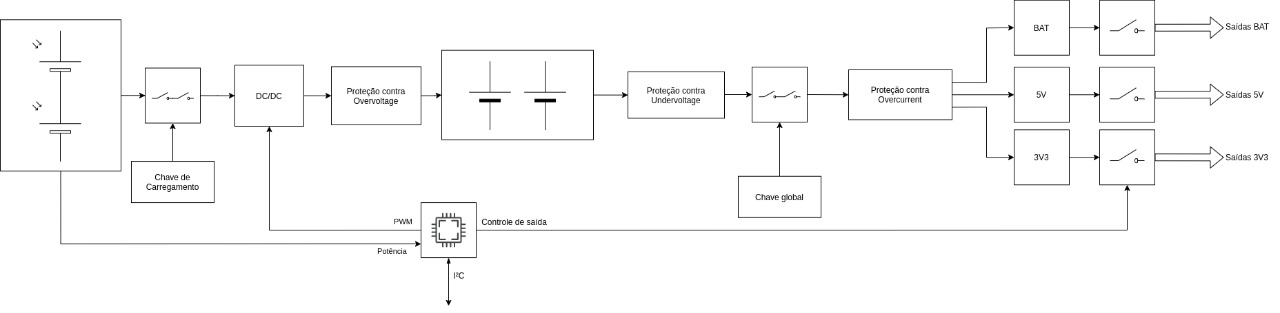
\includegraphics[angle=270,keepaspectratio=true, scale=0.55]{imagens/DiagramaBlocos.jpeg}}
\captionof{figure}{Diagrama de blocos proposto para o EPS}
\label{fig:block_diagram}
\end{minipage}

\subsection*{Tarefas e \textit{Power Budget}}

Após levantar os consumos de cada módulo, o próximo passo é construir um \textit{power budget} baseado nas tarefas que o \textit{cubesat} precisa realizar ao longo de um ciclo.  

Alguns blocos da figura \ref{fig:block_diagram}, tais como as células solares e baterias foram escolhidas baseadas no \textit{power budget} disponível. Segue abaixo o \textit{power budget} estimado para a missão, detalhando cada um dos componentes e seus consumos, baseado nisso, e usando as informações da órbita, é possível determinar o número minímo de baterias e de células solares para conseguir carregar com sucesso o conjunto de baterias durante um ciclo. A figura \ref{fig:power_budget} mostra o \textit{power budget}:

\noindent
\begin{minipage}{\linewidth}
\makebox[\linewidth]{
    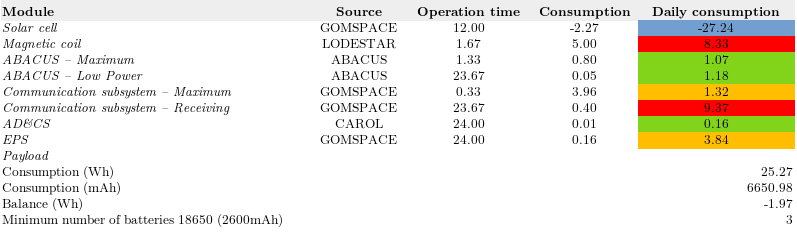
\includegraphics[keepaspectratio=true, scale=0.5]{imagens/powerbudget.png}}
\captionof{figure}{\textit{Power budget} estimado para o EPS}
\label{fig:power_budget}
\end{minipage}

As seguintes premissas foram consideradas na construção dessa tabela:

\begin{enumerate}
    \item O sistema de comunicação irá operar por um período máximo de 20 minutos e permanecerá em modo de recepção durante o restante do ciclo.
    \item O consumo do atuador magnético está modelado para funcionar com pulsos de 1 minuto em potência máxima, é assumido que haverão 100 pulsos durante o ciclo.
    \item O computador de bordo (OBC) estará em modo ativo por no máximo 1 hora e durante o tempo que estiver ocorrendo transmissões, no total de 1 hora e 20 minutos.
    \item Apenas uma das faces do nanossatélite está exposta à radiação solar por vez.
\end{enumerate}


Na coluna \textit{Source} é colocado de onde é vieram as informações a respeito do módulo, onde aparece a GOMSpace é uma fabricante e fornecedora de nanossatélites e componentes em vários mercados, além de ser uma empresa referência no mercado, com vários cases de sucesso, o laboratório LODESTAR tem intenção de compra com a GOMSpace do nanossatélite do primeiro lançamento da missão. O Abacus é um computador de bordo (OBC) fabricado pela Gauss Srl e utilizado para testes no LODESTAR, por ser um OBC multi-propósito ele tem um consumo maior do que os computadores da GOMSpace, o que pode vir a aumentar o nosso saldo no Power Budget. O atuador magnético \cite{unb_mag_actuator} e o ADCS \textit{TODO: ACHAR REFERENCIA} utilizados de referência são de trabalhos desenvolvidos por alunos do laboratório. 


Com esse \textit{power budget}, a menor célular solar (1U) da GOMSPACE é usada como referência. Essa célula solar é capaz de prover até \SI{27}{\watt}. Note que usada apenas essa célula, o \textit{budget} ainda fica com um saldo negativo, o que significa que estamos consumindo menos energia do que a que conseguimos adquirir, porém essa margem ainda é pequena. Portanto, mais células solares devem ser usadas para prover uma quantidade segura de energia.

Conhecer os consumos dos módulos permitiu calcular quantas baterias, aqui estamos utilzando os modelos 18650 como referência, para manter o nanossatelite alimentado durante um ciclo. Os modelos de baterias 18650 são largamente utilizados nos EPS pela padronização de tamanho e segurança. No modelo referência da GOMSPACE temos \SI{2600}{\milli\ampere\hour}, ou seja, para conseguir suprir o consumo de \SI{6650}{\milli\ampere\hour}, pelo menos três dessas baterias.

\section{Circuito de carga da bateria}

Uma das tarefas cruciais para o projeto do circuito de carga da bateria é escolher o conversor DC/DC que fará a interface entre o painel solar e a bateria, o que nos permite aplicar a técnica de MPPT. Para cumprir essa tarefa, foi realizada uma busca pelos conversores disponíveis comercialmente e abaixo apresentaremos os resultados e as métricas utilizadas para escolha.




\section{Solução com controlador integrado}

O uso de um chip independente para a implentação do MPPT traz muitas vantagens com relação a implementação tradicional com componentes discretos. A primeira delas é que isso torna o sistema MPPT complementamente autônomo, isso permite que o aquisição de energia continue mesmo com o esgotamento total das baterias. A segunda é por dispensar recursos do microcontrolador, seja por livrar recursos de algum que desempenha várias funcionalidade ou dispensar um microcontrolador exclusivo para essa tarefa. A terceira está relacionada com a segunda, que é o \textit{footprint} bem reduzido no projeto final da PCB, pois estamos dispensando vários componentes discretos.





	\chapter{Resultados} \label{resultados}

\section{Modelos de referência}
O painel solar escolhido para as simulações é um modelo da GOMSpace, o NanoPower P110 \cite{pv_gomspace_datasheet}, a tabela \ref{pv_specs_table} detalha as suas especificações técnicas. Para simular da melhor forma o comportamento do painel nas simulações SPICE, utilizaremos o modelo de aproximação pelos dados do datasheet, conforme apresentado na revisão teórica.

\begin{table}[H]
\centering
\caption{Especificações do NanoPower P110}
\label{pv_specs_table}
\begin{tabular}{|l|l|l|l|l|l|} 
\cline{2-6}
\multicolumn{1}{c|}{} & Condition                  & \multicolumn{1}{c|}{Min} & \multicolumn{1}{c|}{Typ} & \multicolumn{1}{c|}{Max} & Unit  \\ 
\hline
Voltage               & Full Sunlight in LEO       & 4.64                     & -                        & 4.84                     & V     \\ 
\hline
Current               & Current at optimal voltage & 490                      & -                        & 508                      & mA    \\ 
\hline
Power                 & Maximum power              & 2270                     & -                        & 2400                     & mW    \\ 
\hline
Efficiency            &                            & 29.8                     & 30                       & 30.2                     & \%    \\
\hline
Temperature coefficient &                            & 0.21                     & 0.233                       & 0.25                     & \%/ºC    \\
\hline
\end{tabular}
\end{table}

\noindent
\begin{minipage}{\linewidth}
\makebox[\linewidth]{
    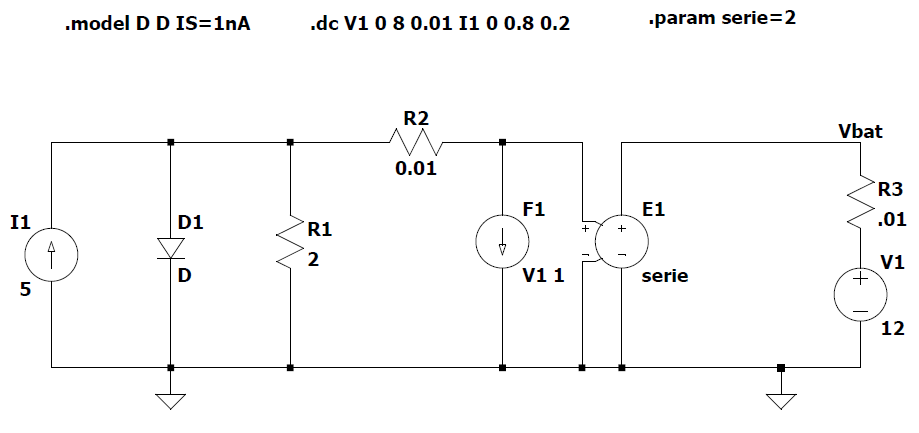
\includegraphics[keepaspectratio=true, scale=0.55]{imagens/PV_model_circuit.png}}
\captionof{figure}{Circuito equivalente para o painel solar}
\label{fig:model_pv_circuit}
\end{minipage}

\noindent
\begin{minipage}{\linewidth}
\makebox[\linewidth]{
    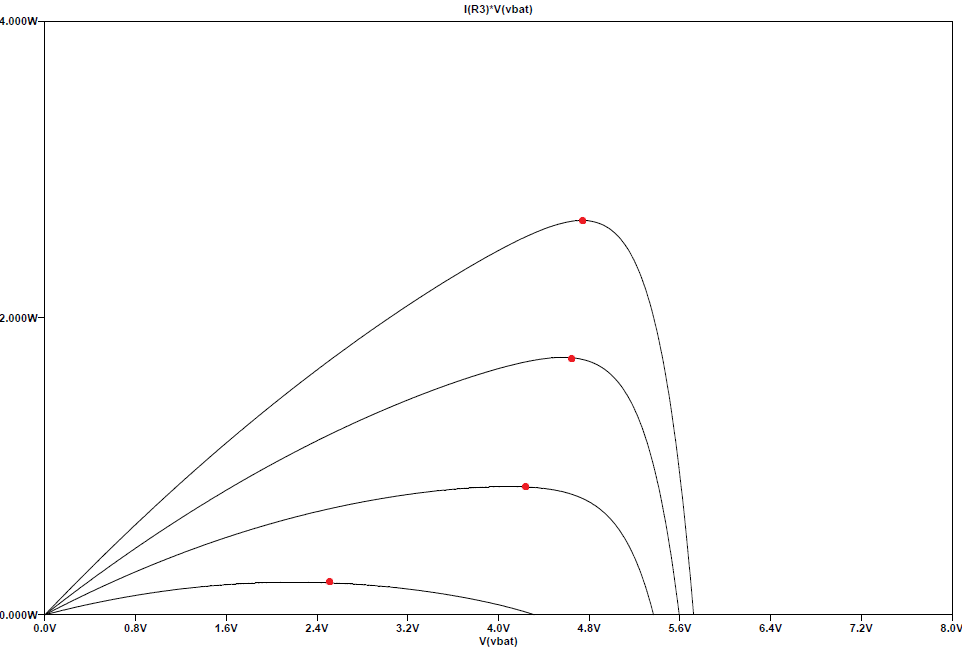
\includegraphics[keepaspectratio=true, scale=0.55]{imagens/PV_model_traces_mpps.png}}
\captionof{figure}{Gráfico de tensão na bateria x potência entregue}
\label{fig:model_pv_traces}
\end{minipage}

No circuito da figura \ref{fig:model_pv_circuit}, além do modelo da célula solar foi colocado um modelo simplificado de bateria consistindo de um fonte de tensão e resistor em série. As fontes lineares dependentes foram adicionadas para simular as células conectadas em série, no caso do painel NanoPower P110 trata-se de duas células 3G30A SCA.

No gráfico \ref{fig:model_pv_traces}, cada uma das curvas dispostas representam irradiações solares distintas, atráves de uma simulação \textit{DC sweep}, alterando as correntes de entrada. A medida que a irradiação solar aumenta, a curva I-V aumenta a sua área e os pontos de máxima potência, marcados em vermelho, se modificam com a tensão de saída no painel solar, o que mostra a necessidade de trabalhar sempre no ponto de máxima potência.  

Para efeitos de simplificação dos esquemáticos, o modelo apresentado estará representado dentro de um modelo customizado no simulador LTSpice chamado de Model\_PV.

Para as baterias, o nosso modelo de referência \cite{battery_gomspace_datasheet} é a bateria Ion-lítio NanoPower 18650 de 2600 mAh. Porém, na questão das baterias, existe uma complexidade adicional, conforme vimos no histórico das missões anteriores, a quantidade e arranjo das células podem variar e isso afeta a condição de carregamento das baterias, por esse motivo, como referência nas simulações, estaremos padronizando a tensão de carregamento na mesma utilizada pelo EPS da GOMSpace, modelo NanoPower P31u \cite{eps_gomspace_datasheet}, que é de 5V.

Para os conversores e controladores, que são os alvos do trabalho, estaremos utilizando os modelos SPICE, fornecidos pelas próprias fabricantes dos chips, sem nenhuma alteração ou customização. 

\subsection*{Cenários de simulação}

Para cada conversor, além do cenário em operação normal, serão apresentados os seguintes cenários:
\begin{itemize}
    \item Transiente da tensão de entrada de 0V até a tensão de operação máxima. Com esse cenário, avalia-se quanto de tensão na entrada é preciso para que o conversor forneça a saída regulada na tensão desejada.
    \item Chaveamento entre desligado e ligado. Nesse cenário, avalia-se a resposta do conversor ao degrau, ou seja, o transiente de quanto o conversor é ligado, o que se traduz em um baixo tempo de resposta, ou seja, o tempo necessário para que a tensão na saída esteja estabilizada é pequeno.
    \item Alterações na carga durante a simulação já com o circuito no estado estável. Uma carga extra será inserida no meio da simulação. Nesse cenário, estamos interessados na resposta do conversor a essa situação. O objetivo é saber quanto tempo é necessário para restaurar a operação normal e o quanto de queda de tensão está presente. 
\end{itemize}


\section{Topologia discreta}

\subsection*{LM2735}

\noindent
\begin{minipage}{\linewidth}
\makebox[\linewidth]{
    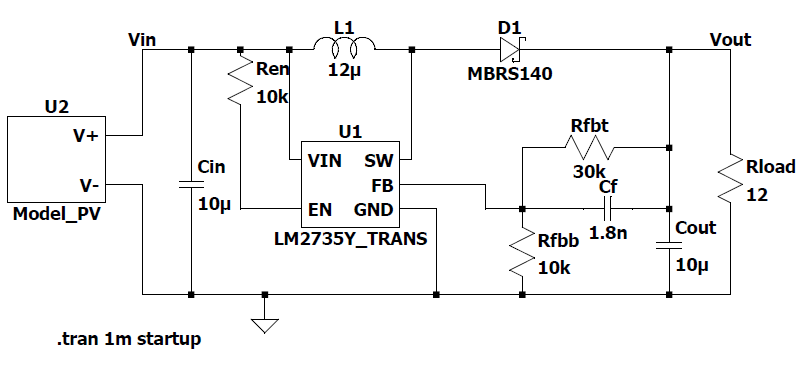
\includegraphics[keepaspectratio=true, scale=0.75]{imagens/LM2735/LM2735_stock_05.png}}
\captionof{figure}{Circuito do LM2735 em condições normais}
\label{fig:lm2735_stock}
\end{minipage}

O LM2735 \cite{lm2735_datasheet} é um conversor DC-DC fabricado pela Texas Instruments, que pode ser usado na configuração Boost ou SEPIC. É um conversor com um \textit{pinout} relativamente pequeno, pois muitas das suas funções são internas e fixas, conforme definido pelo fabricante. Alguns exemplos são o \textit{soft-start} interno e fixo em 4 ms, compensação interna, a frequência de chaveamento fixa em 520 kHz, todas essas funcionalidades internas e fixas poupam a existência de pinos de configuração e ajuda a diminuir o espaço consumido pelo circuito integrado dentro da PCB. O conversor conta ainda com a presença um pino de \textit{Enable} ativo alto. A tabela \ref{lm2735_specs_table} mostra as especificações de operação.

\begin{table}
\centering
\caption{Especificações do LM2735Y}
\label{lm2735_specs_table}
\begin{tabular}{|l|l|l|l|l|} 
\cline{2-5}
\multicolumn{1}{c|}{} & \multicolumn{1}{c|}{Min} & \multicolumn{1}{c|}{Typ} & \multicolumn{1}{c|}{Max} & Unit  \\ 
\hline
Input                 & 2.7                      & -                        & 5.5                      & V     \\ 
\hline
Output                & 3                        & -                        & 24                       & V   \\ 
\hline
Switch current                & -                        & -                        & 2.1                      & A   \\ 
\hline
Switching Frequency   & 360                        & 520                      & 580                        & kHz   \\
\hline
Duty Cycle   & 2                        & 99 ($T_{J}$ = 25ºC)                      & 91                        & \%   \\
\hline
\end{tabular}
\end{table}

\noindent
\begin{minipage}{\linewidth}
\makebox[\linewidth]{
    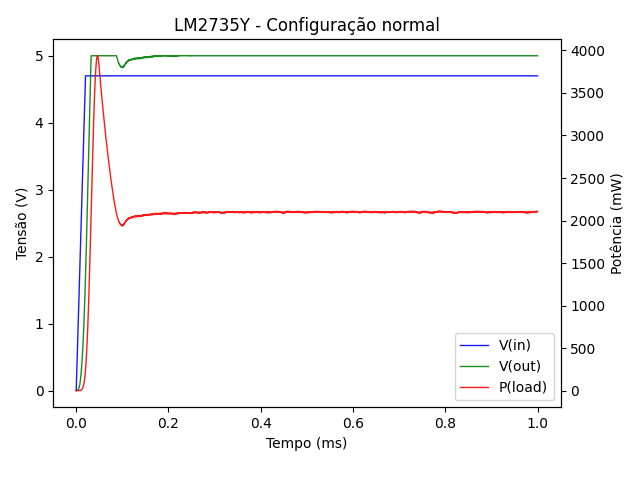
\includegraphics[keepaspectratio=true, scale=1]{imagens/LM2735/5V@05A.png}}
\captionof{figure}{Resposta do LM2735 em condições normais}
\label{fig:lm2735_traces_stock}
\end{minipage}

Um ponto fundamental de vantagem do regulador chaveado frente ao regulador linear é a eficiência energética. Dado que um regulador chaveado consegue chegar a eficiência de potência da ordem de 90\%. A eficiência é importantíssima no cubesat, que está em um ambiente com fonte limitada de energia, fonte essa que também é intermitente: depende do satélite estar ou não em eclipse.

Analisando a resposta da figura \ref{fig:lm2735_traces_stock}, essa configuração \ref{fig:lm2735_stock} atingiu uma eficiência de 87.8\%, com aproximadamente 2.115 W sendo entregues para a carga.
A tensão $V_{pp}$ de ripple na saída ficou em 12.64 mV, dentro da faixa de valores esperada. Vale ressaltar que esse resultado considera a frequência fixa de chaveamento do conversor de 520 kHz, porém a Texas em seu datasheet explicita que esse valor é válido para $T_{J}$ = 25 ºC, para a faixa de temperaturas de operação que é $T_{J}$ entre -40 ºC e 125 ºC, essa frequência pode oscilar entre 360 e 680 kHz. Portanto, o fato do modelo SPICE não simular os efeitos da temperatura no circuito coloca essa limitação.

\noindent
\begin{minipage}{\linewidth}
\makebox[\linewidth]{
    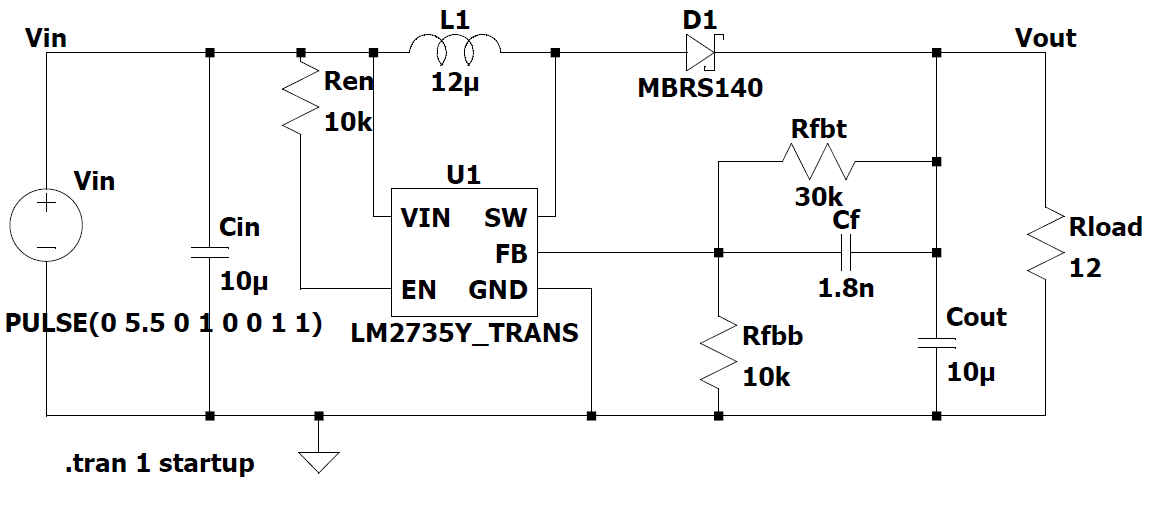
\includegraphics[keepaspectratio=true, scale=0.55]{imagens/LM2735/LM2735_transient_05.png}}
\captionof{figure}{Circuito do LM2735 em transiente de tensão}
\label{fig:lm2735_transient}
\end{minipage}

\noindent
\begin{minipage}{\linewidth}
\makebox[\linewidth]{
    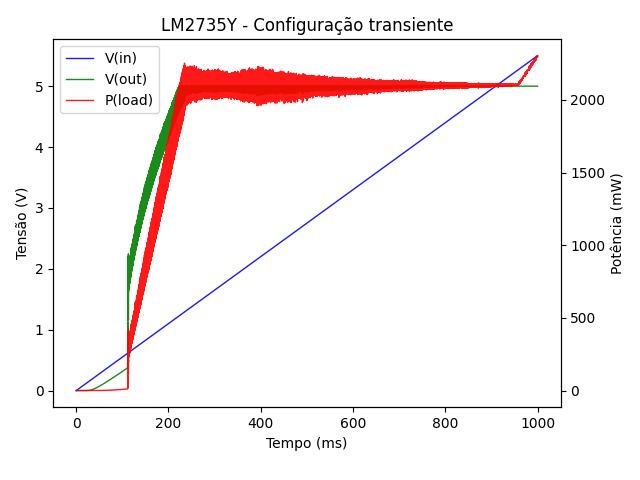
\includegraphics[keepaspectratio=true, scale=1]{imagens/LM2735/5V@05A_transient.png}}
\captionof{figure}{Resposta do LM2735 em transiente de tensão}
\label{fig:lm2735_traces_transient}
\end{minipage}

A figura \ref{fig:lm2735_traces_transient} mostra a resposta quando temos o transiente de tensão aplicado, para isso substituimos o painel solar por uma fonte de tensão do tipo PULSE, que foi programada para executar uma rampa de 0 até 7 V em 1 s. Observa-se que quando a tensão de entrada ultrapassa o valor de aproximadamente 1.3V já é possível observar uma tensão na saída, porém com uma tensão de \textit{ripple} bastante elevada de 330.14 mV, fora da tolerância. Quando a tensão mínima de entrada do conversor (2.7 V) é atingida, é possível obter uma tensão de saída próxima do alvo de 5 V e com a tensão de \textit{ripple} dentro da tolerância de 5\% do valor da saída, com 115.14 mV. Esse \textit{ripple} vai diminuindo a medida que a tensão na entrada aumenta para a tensão esperada do ponto de máxima potência do painel solar e a para as tensões de entrada superiores as esperadas para o painel, a saída se satura em aproximadamente 5.1 V.

\noindent
\begin{minipage}{\linewidth}
\makebox[\linewidth]{
    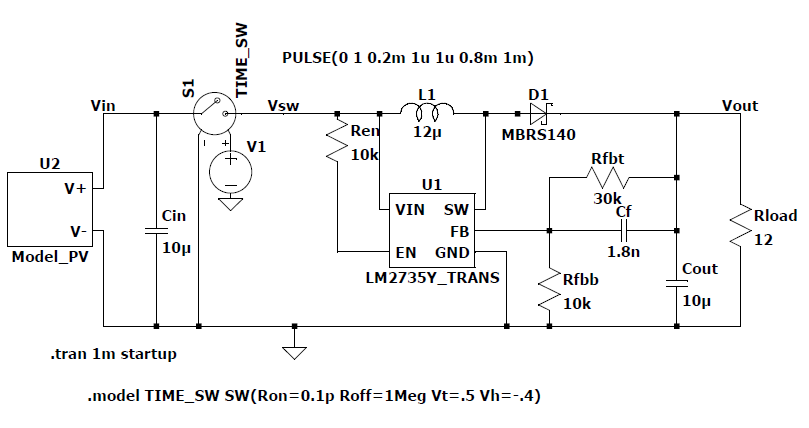
\includegraphics[keepaspectratio=true, scale=0.75]{imagens/LM2735/LM2735_switch_05.png}}
\captionof{figure}{Circuito do LM2735 com chaveamento}
\label{fig:lm2735_switch}
\end{minipage}

\noindent
\begin{minipage}{\linewidth}
\makebox[\linewidth]{
    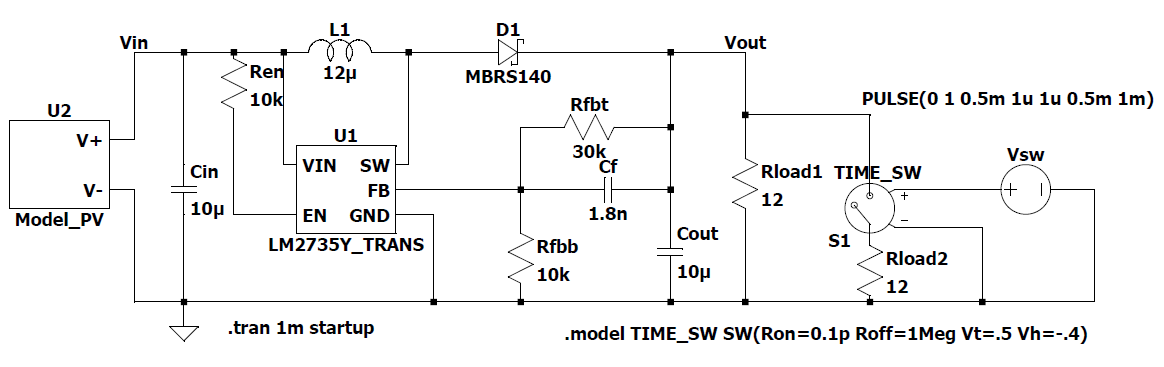
\includegraphics[keepaspectratio=true, scale=0.55]{imagens/LM2735/LM2735_current_05.png}}
\captionof{figure}{Circuito do LM2735 com alteração na carga}
\label{fig:lm2735_current}
\end{minipage}

\noindent
\begin{minipage}{\linewidth}
\makebox[\linewidth]{
    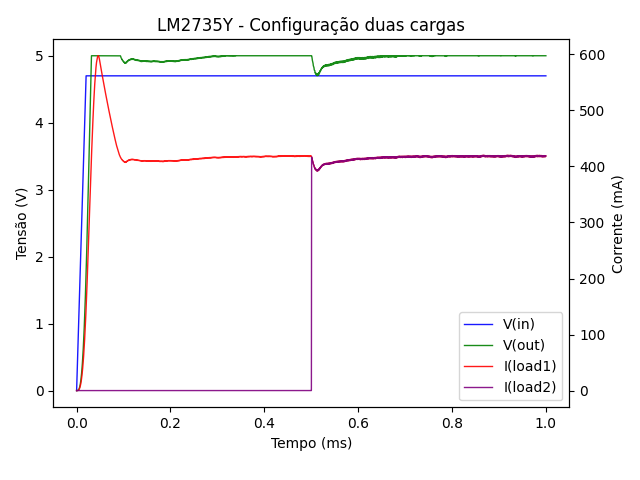
\includegraphics[keepaspectratio=true, scale=1]{imagens/LM2735/5V@05A_current.png}}
\captionof{figure}{Resposta do LM2735 com alteração na carga}
\label{fig:lm2735_traces_current}
\end{minipage}

As figuras \ref{fig:lm2735_current} e \ref{fig:lm2735_traces_current} mostram a resposta do conversor quando uma segunda carga resistiva de 5 $\Omega$ é inserida no circuito, a chave foi programada para ligar em t=0.5 ms, observa-se que o conversor consegue retomar a situação estável em 0.155 ms após o chaveamento da segunda carga, com uma queda de tensão na saída de 0.32V. O tempo de resposta foi bastante parecido com o chaveamento entre ligado e desligado (única carga de 12 $\Omega$) que foi de 0.191 ms, conforme figura \ref{fig:lm2735_traces_switch}, porém a tensão de \textit{ripple} na saída é afetada, passando de 10.05 mV para 28.31 mV, mais do que o dobro da tensão com apenas uma carga.

\noindent
\begin{minipage}{\linewidth}
\makebox[\linewidth]{
    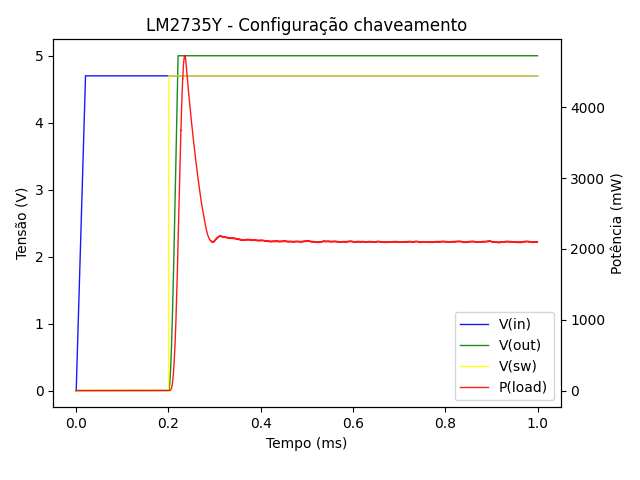
\includegraphics[keepaspectratio=true, scale=1]{imagens/LM2735/5V@05A_switch.png}}
\captionof{figure}{Resposta do LM2735 com chaveamento}
\label{fig:lm2735_traces_switch}
\end{minipage}

\section{Controlador Integrado}

\subsection*{SPV1040}

Para a solução integrada, utilizaremos de referência o SPV1040 \cite{spv1040_datasheet} da ST Microelectronics, o mesmo utilizado na missão ESTCube-1. 

Conforme explicado no capítulo \ref{desenvolvimento}, o SPV1040 é um controlador completo, dessa forma, o \textit{Duty Cycle} é internamente controlado pelo algoritmo de MPPT, o que no caso desse componente é o algoritmo Pertuba e Observa. A tensão de entrada $V_{in}$ opera entre os valores de 0.3 e 5.5 V, o é que suficiente para o painel solar escolhido e a frequência de chaveamento é fixa em 100 kHz. Além de já fornecer a saída regulada, possui também proteção contra superaquecimento e sobrecorrente. Dependendo da configuração, o \textit{datasheet} mostra que a eficiência dele pode chegar em até 95\%, sendo extremamente indicado para essas situações onde é preciso lidar com tensões de entrada baixas. 

O dispositivo fornece saída regulada de tensão e corrente detectando a tensão $V_{CTRL}$ de \textit{feedback} do divisor de resistor externo, que define a tensão na bateria, e pela queda de tensão no resistor de detecção externa $R_{S}$, respectivamente.

Existem 5 modos de operação possíveis para o controlador:
\begin{enumerate}
    \item Start-up: Quando a tensão de saída $V_{out}$ está acima 0.8 e abaixo 2 V, o dispositivo entra no modo start-up, pois nessa condição a polarização dos MOSFET's de compensação (\textit{BIAS}) ainda não é garantida. Em tais condições, o transistor canal N é forçado a ligar com um duty cycle fixo.
    \item MPPT: Uma vez que o dispositivo saiu do modo start-up, o dispositivo entra no modo MPPT, que utiliza o algoritmo Perturba e Observa.
    \item Shutdown: Modo com o menor consumo energético possível, ativado quando o pino XSHUT está em LOW.
    \item Burst: O modo burst é a transição para o modo sleep-in, o conversor DC-DC começa a operar em frequências cada vez mais lentas. O modo burst atua quando a tensão de saída atinge a tensão da bateria, o pino MPP-SET abaixa de 0.45V ou a corrente de saída atinge o seu valor máximo.
    \item Sleep-in: Nesse modo, nenhuma corrente é fornecida para a carga e esse estado permanece até que a condição que colocou o dispositivo em Sleep-in não esteja mais presente.
\end{enumerate}

A figura \ref{fig:spv1040_block} mostra o diagrama de blocos do dispositivo e a figura \ref{fig:spv1040_sample} mostra o esquemático do circuito necessário para uma saída de 3.8 V com 500 mA, o equivalente para uma bateria de referência da GOMSpace.

\noindent
\begin{minipage}{\linewidth}
\makebox[\linewidth]{
    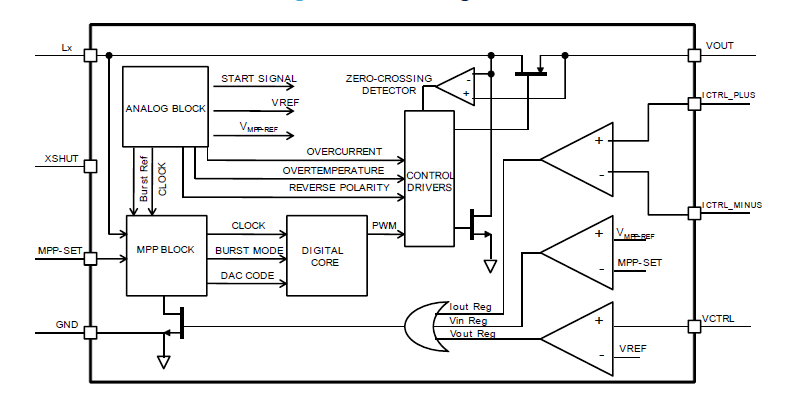
\includegraphics[keepaspectratio=true, scale=0.8]{imagens/SPV1040/SPV1040_block.png}}
\captionof{figure}{SPV1040: Diagrama de blocos}
\label{fig:spv1040_block}
\end{minipage}

\noindent
\begin{minipage}{\linewidth}
\makebox[\linewidth]{
    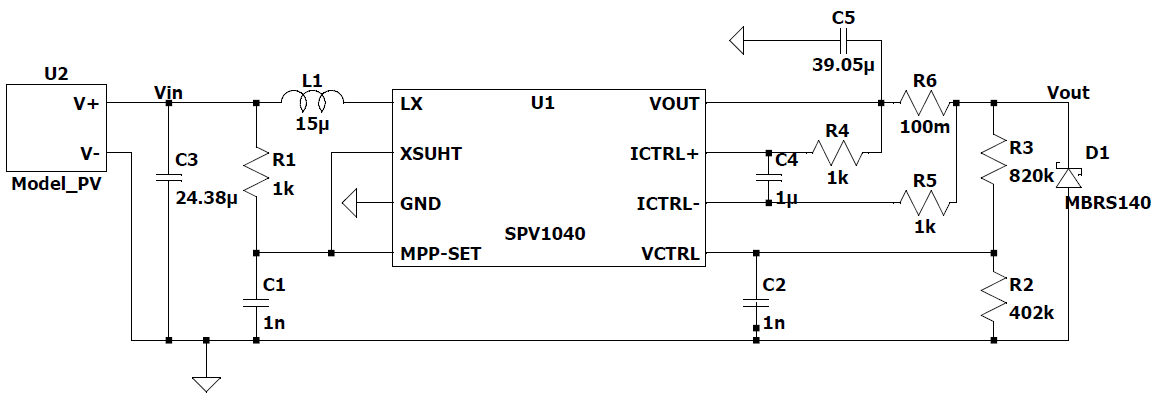
\includegraphics[keepaspectratio=true, scale=0.75]{imagens/SPV1040/SPV1040_sample.png}}
\captionof{figure}{SPV1040 configurado para 3.8 V @ 500 mA}
\label{fig:spv1040_sample}
\end{minipage}
	%Usar \chapter*{Título do Capítulo} faz com que o capítulo não seja numerado
\chapter{Conclusão} \label{conclusao}

Este trabalho apresentou um estudo de viabilidade e proposta de topologia para o futuro módulo EPS - \textit{Electrical Power System} para os \textit{cubesats} da constelação Alfacrux da Universidade de Brasília (UnB). 

Inicialmente foi realizada uma conceituação básica do tema, apresentando o projeto Alfacrux em seguida do conceito de \textit{cubesat} e seus módulos, como o módulo EPS se encaixa no \textit{cubesat} e qual papel desempenha. Em seguida, foram apresentados os requisitos propostos para o módulo e quais os objetivos desse trabalho diante desses requisitos.

Na revisão téorica, abordou-se os principais conceitos para o entendimento da topologia proposta, apresentou-se a especificação \textit{cubesat}, o funcionamento básico de um painel solar, os dispositivos de conversão DC-DC, a técnica MPPT - \textit{Maximum Peak Point Tracking} e os dois algoritmos mais utilizados para executá-la.

O desenvolvimento inicia apresentando um \textit{background} de missões anteriores de quatro nanossatélites distintos e quais soluções eram utilizadas para os módulos EPS. Após isso, é mostrado o levantamento que foi realizado em termos dos \textit{payloads}, os seus consumos e tarefas desempenhadas por eles e como que esse consumo energético está ligado ao dimensionamento do EPS, consolidando os objetivos especifícos 1, 2 e 3.

A proposta foi dividida em duas topologias, uma com os componentes discretos, a qual foi simulada e construída, de acordo com os modelos de referência apresentados para placa solar, baterias e EPS, com o conversor DC-DC LM2735Y da Texas Instruments, que tem as vantagens de ser um conversor mais simples, com menos configurações, ocupando pouco espaço de PCB, contudo atingindo uma alta eficiência. Para a segunda topologia com o controlador MPPT, foi apresentado o SPV1040, o mesmo utilizado na missão ESTCube-1, as suas especificações, modos de operação e um circuito projetado para o cenário proposto conforme explicado nos modelos de referência, porém que não foi possível executar simulações pela ausência de modelos SPICE para o componente, dessa forma, o objetivo especifíco 4 foi cumprido apenas parcialmente.

No fim, ambas as topologias são capazes de atender os aspectos técnicos necessários para o EPS, conforme observado na tabela \ref{comparison_specs_table} que coloca lado a lado as especificações de ambos os dispositivos, em seguida, as tabelas \ref{lm2735_bom_table} e \ref{spv1040_specs_table} mostram uma possível lista de materiais requeridos por cada uma das implementações.

Portanto, visando os critérios de um menor número de componentes, o que, por sua vez, diminui o esforço para integração e de programação de microcontroladores, um menor espaço ocupado em PCB e um menor custo de implementação, a topologia com o circuito integrado de controlador MPPT é a mais recomendada.

\subsection*{Recomendações de trabalhos futuros}

Os trabalhos futuros são de extrema importância para a continuidade do projeto, existem diversas formas para reforçar e validar o que foi exposto nesse trabalho, sendo a mais latente delas o desenvolvimento de um modelo funcional para o chip SPV1040T, o que permitiria uma comparação direta com as simulações do conversor da Texas. Outras possibilidades envolvem simular o comportamento do conversor LM2735Y para mais cenários e configurações de carregamento distintas, incorporar ao cálculo de \textit{power budget} um modelo orbital mais preciso, a exemplo do que é usado no nanossatélite OUFTI-Next \cite{orbit_dynamics_ref}. Todas essas tarefas podem vir a incorporar dados valiosos ao trabalho aqui iniciado. 


% Além das próximas tarefas naturais do projeto que envolvem a integração desses componentes do circuito de carga da bateria ao \textit{layout} de PCB para o módulo EPS, que já se encontra em fase de projeto e desenvolvimento pelo aluno Luiz Antônio, com a orientação do Professor Daniel Café, trabalho acompanhado por mim. 
 
		
	\bibliographystyle{abnt-num} % estilo bibliográfico ABNT numérico
	%\bibliographystyle{abnt-alf} % estilo bibliográfico ABNT alfabético
	%\bibliographystyle{sbc}  % estilo bibliográfico da Sociedade Brasileira de Computação (SBC)
	
	%\renewcommand{\bibname}{REFERÊNCIAS BIBLIOGRÁFICAS} %Define o Caption da seção de bibliografia
	%\addcontentsline{toc}{chapter}{REFERÊNCIAS BIBLIOGRÁFICAS}
	
	%não pode ter espaço entre os nomes dos arquivos bib
	\bibliography{referencias}
	
	\chapter*{Apêndices}

\noindent
\begin{minipage}{\linewidth}
\makebox[\linewidth]{
    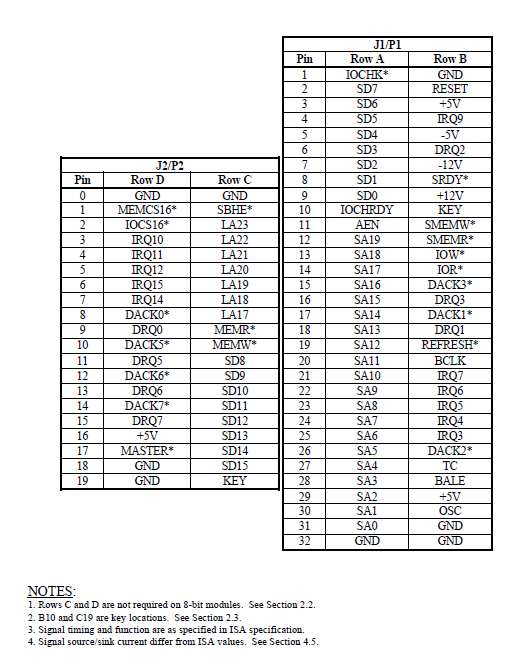
\includegraphics[keepaspectratio=true, scale=1]{imagens/apendices/pc104-signal-assignments-table.PNG}}
\captionof{figure}{Tabela de atribuições de pinos nos barramentos PC/104 8 e 16-bits.}
\label{pc104_signal_assignments_table}
\end{minipage}

\end{document}

